% !TeX spellcheck = en_US
\documentclass[conference]{IEEEtran}

% *** GRAPHICS RELATED PACKAGES ***
%
\usepackage[pdftex]{graphicx}
% declare the path(s) where your graphic files are
\graphicspath{{./figures/}}
% and their extensions so you won't have to specify these with
% every instance of \includegraphics
\DeclareGraphicsExtensions{.pdf,.jpeg,.png}

% *** MATH PACKAGES ***
%
\usepackage{amsfonts,amsmath,amssymb} % Mathematical symbols.

% correct bad hyphenation here
\usepackage{listings}
\usepackage{cite}
%\usepackage{caption}
\hyphenation{UPPAAL}

\usepackage{url}

\newcommand{\framework}[0]{\text{Gamma Framework}}
\newcommand{\Framework}[0]{\text{Gamma Framework}}
\renewcommand{\gamma}[0]{\text{Gamma}}
\renewcommand{\Gamma}[0]{\text{Gamma}}
\newcommand{\Yakindu}{\textsf{Yakindu}}

\newcommand{\eg}{e.g., }
\newcommand{\ie}{i.e., }

\newcommand{\RNum}[1]{\uppercase\expandafter{\romannumeral #1\relax}}
\newcommand{\ptolemy}{Ptolemy \RNum{2}}

\newcommand{\specialcell}[2][c]{%
	\begin{tabular}[#1]{@{}c@{}}#2\end{tabular}}

\newenvironment*{mytable}[3]{
	% #1: caption, #2: cimke, #3: oszlopdef		 
	\begin{table}[htbp]	
		\caption{#1}          
		\label{tab:#2}            
		\center%
		\begin{tabular}{#3}
		}
		{
		\end{tabular}
	\end{table}
}

% Define Language
\lstdefinelanguage{Gamma}
{
	% list of keywords
	morekeywords={
		const,
		integer, 
		natural,
		interface,
		extends,
		in,
		out,
		inout,
		event,
		import,
		package,
		statechart,
		rate,
		var,
		transition,
		from,
		to,
		region,
		initial,
		shallow,
		deep,
		history,
		state,
		entry,
		exit,
		assign,		
		sync,
		cascade,
		async, 
		of,
		port,
		provides,
		requires,
		component,
		bind,
		->,
		channel,
		-o)-,
		any,
		run,
		full,
		step,
		reset,
		priority,
		capacity,
		clock,
		s,
		ms,
		when,
		queue
	},
	sensitive=true, % keywords are not case-sensitive
	morecomment=[l]{//}, % l is for line comment
	morecomment=[s]{/*}{*/}, % s is for start and end delimiter
	morestring=[b]" % defines that strings are enclosed in double quotes
}

% Define Colors
\usepackage{color}
\definecolor{eclipseBlue}{RGB}{42,0.0,255}
\definecolor{eclipseGreen}{RGB}{63,127,95}
\definecolor{eclipsePurple}{RGB}{127,0,85}

\definecolor{lightgray}{rgb}{0.95,0.95,0.95}
\lstset{
	basicstyle=\footnotesize, % print whole listing small
	keywordstyle=\color{black}\bfseries, % bold black keywords
	identifierstyle=, % nothing happens
	% default behavior: comments in italic, to change use
	% commentstyle=\color{green}, % for e.g. green comments
	stringstyle=\scriptsize,
	showstringspaces=false, % no special string spaces
	backgroundcolor = \color{white},
	aboveskip=1.5\medskipamount,	
	columns=flexible,
	keepspaces=true,
	escapeinside={(*@}{@*)},
	captionpos=b,
	breaklines=true,
	frame=single,
	float=!ht,
	literate=*
	{á}{{\'a}}1	{é}{{\'e}}1	{í}{{\'i}}1	{ó}{{\'o}}1	{ö}{{\"o}}1	{ő}{{\H{o}}}1	{ú}{{\'u}}1	{ü}{{\"u}}1	{ű}{{\H{u}}}1
	{Á}{{\'A}}1	{É}{{\'E}}1	{Í}{{\'I}}1	{Ó}{{\'O}}1	{Ö}{{\"O}}1	{Ő}{{\H{O}}}1	{Ú}{{\'U}}1	{Ü}{{\"U}}1	{Ű}{{\H{U}}}1
}


% Set Language
\newcommand{\setGammaSyntax}{
	\lstset {
		language={Gamma},
		basicstyle=\footnotesize, % Global Code Style
		captionpos=b, % Position of the Caption (t for top, b for bottom)
		extendedchars=true, % Allows 256 instead of 128 ASCII characters
		tabsize=2, % number of spaces indented when discovering a tab 
		columns=fixed, % make all characters equal width
		keepspaces=true, % does not ignore spaces to fit width, convert tabs to spaces
		showstringspaces=false, % lets spaces in strings appear as real spaces
		breaklines=true, % wrap lines if they don't fit
		frame=trbl, % draw a frame at the top, right, left and bottom of the listing
		frameround=tttt, % make the frame round at all four corners
		framesep=4pt, % quarter circle size of the round corners
		%		numbers=left, % show line numbers at the left
		%		numberstyle=\tiny\ttfamily, % style of the line numbers
		commentstyle=\color{eclipseGreen}, % style of comments
		keywordstyle=\color{black}\bfseries, % style of keywords
		stringstyle=\color{eclipseBlue}, % style of strings
	}
}

\begin{document}
\setGammaSyntax
\title{Mix and Match Composition in the \\ Gamma Framework}

% author names and affiliations
% use a multiple column layout for up to three different
% affiliations
\author{\IEEEauthorblockN{Bence Graics, Vince Moln\'ar}
\IEEEauthorblockA{Budapest University of Technology and Economics, \\
Department of Measurement and Information Systems \\
Budapest, Hungary \\
Email: \texttt{bence.graics@gmail.com},  \texttt{molnarv@mit.bme.hu}}

}

% make the title area
\maketitle

% !TeX spellcheck = en_US
% As a general rule, do not put math, special symbols or citations
% in the abstract
\begin{abstract}

The \gamma\ Statechart Composition Framework is a modeling tool that supports the hierarchical composition of statechart components with well-defined compositonal semantics, as well as source code generation and formal verification. The purpose of the framework is to provide common ground for modeling and verification tools, as well as to support component-based system design building on existing statechart modeling tools. Currently, the framework has a single composition semantics, which executes the components in a lockstep fashion. This paper presents a new composition language for the \gamma\ Framework, adding support for two more semantics. Asynchronous-reactive semantics supports the proper abstraction of distributed communication, synchronous-reactive supports the modeling of highly synchronous communication, and cascade composition is a sequential decomposition of a single function. 
\end{abstract}
% For peer review papers, you can put extra information on the cover
% page as needed:
% \ifCLASSOPTIONpeerreview
% \begin{center} \bfseries EDICS Category: 3-BBND \end{center}
% \fi
%
% For peerreview papers, this IEEEtran command inserts a page break and
% creates the second title. It will be ignored for other modes.
\IEEEpeerreviewmaketitle

\section{Introduction}
\label{sec:introduction}
Statecharts \cite{Harel:1987:SVF:34884.34886} are a widely used formalism to describe the behavior of reactive systems, which process stimuli from the environment and react with respect to their internal states. Statecharts introduce complex elements to aid the modeling of such systems, e.g., variables, hierarchical state refinement, history states and complex transitions (e.g., inner transitions).

The requirements such systems have to meet are getting more complex, which can result in very large system models, hindering verifiability, maintenance and extensibility. A well-known solution for managing complexity is decomposition. In case of statecharts, one way of decomposition is to define individual reactive components that, by means of communication, realize a more complex behavior. There are a number of modeling tools that aim to support this practice with various model-driven software development techniques such as code generation and verification.

The \gamma\ Statechart Composition Framework is one such tool, providing a layer for composing individual statechart components (possibly coming from other tools) while extending the capabilities of automatic code generation and verification and validation (V\&V). Functionalities of the \gamma\ Framework as well as a case study are presented in \cite{graics-bence-bsc}. In this paper, we propose a new composition language for \gamma\ that enables the hierarchical mixing of different composition semantics, with a focus on features and modeling aspects.

\textbf{Asynchronous-reactive:} Such models represent a set of components that are executed independently. Asynchronous components communicate by means of messages and message queues. This semantics is convenient when decomposition is both logical and physical, \eg for distributed controllers.
	
\textbf{Synchronous-reactive:} A synchronous model represents a coherent unit consisting of strongly coupled but concurrent components which communicate in a synchronous manner using signals. This semantics is suitable for the logical decomposition of synchronous systems or the modeling of hardware-related designs.
	
\textbf{Cascade:} Cascade models represent a set of filters that are applied sequentially to derive an output from an input. This variant supports the design of adapters, runtime monitors and units with a batch-like execution.

%The main advantage of the new language is the ability to mix the above semantics hierarchically, using the most suitable variant for the different levels of decomposition.

The rest of the paper is structured as follows. Section~\ref{sec:related-tools} presents a short summary of tools that inspired the design of the composition language. The elements of the language itself and an example are introduced in Section \ref{sec:composition-language}. Finally, Section \ref{sec:conclusion} provides concluding remarks and ideas for future work.

\section{Related Tools}
\label{sec:related-tools}

We present three tools that also support the \emph{mixing of different composition semantics} for component-based systems.

\ptolemy\footnote{\url{http://ptolemy.eecs.berkeley.edu/}} \cite{ptolemy,ptolemy2} is an open-source framework aiming to support
the modeling of hierarchical composite systems with numerous component variants and communication semantics. Communication semantics are determined by \emph{directors}, which are responsible for defining a \emph{model of computation} on a particular hierarchy level. Various directors (e.g., process network, synchronous data flow
or synchronous reactive) can be combined through different hierarchy levels, facilitating the design of complex model behavior. One of the main strengths of Ptolemy II is its simulation capability. However, source code generation and formal verification are not supported.

BIP\footnote{\url{http://www-verimag.imag.fr/Rigorous-Design-of-Component-Based.html?lang=en}} \cite{bip,bip3} is a modeling framework that focuses on the formal definition of heterogeneous systems.
BIP offers a language to define hierarchical composite models, where the interactions of constituent components are based on \emph{synchronization}. BIP defines a clear operational semantics that describes the behavior for both atomic components (transition system model) and compound components (rigorous rules for component interactions). Moreover, BIP offers a comprehensive tool set, which provides model transformers for third-party models, code generators, and formal
verification capabilities.

Stateflow\footnote{\url{https://www.mathworks.com/products/stateflow.html}} \cite{stateflow} is a commercial framework that supports the modeling of
reactive systems. Stateflow supports the design of
statecharts and provides various scheduling
algorithms. Furthermore, Stateflow supports the simulation, validation and verification of models as well as source code generation. Stateflow is a mature commercial software product with professional
support. As such, the possibilities of extending or integrating it with other software is limited. Furthermore, it is very expensive even for research purposes.

Gamma was designed to provide an extensible framework for the design of statechart-based composite systems, inspired by the merits and limitations of the presented tools. 


%\section{The Gamma Statechart Language}
%\label{sec:statechart-language}
%The goal of the \gamma\ statechart language is to support the rigorous design of reactive
%systems while providing conventional facilities of modern statechart languages. To support
%strictness, a well-defined semantics is needed. The language is given a denotational semantics
%described in \cite{graics-bence-bsc} by mapping gamma model constructions to the elements of a formal timed
%automaton implementation. The most important elements of the language are presented in this section using a simple \emph{timer} statechart capable of measuring time.
%
%The execution of the statechart starts in the \emph{Idle} state, with the \emph{elapsedTime} variable set to $-1$. When a \emph{start} event is received on its \emph{control} port, it changes its state to \emph{Measuring}, where the incoming \emph{tick} events are counted using a loop transition. When a \emph{stop} event is received, the statechart goes back to state \emph{Idle} while storing the elapsed number of ticks in variable \emph{elapsedTime}. The measuring process can be restarted with an additional \emph{start} event.
%\begin{lstlisting}
%statechart Timer [
%  // Port for communication
%  port control : provides Control
%] {
%  var elapsedTime : integer := -1
%  // Transition without trigger
%  transition from Initial to Idle 
%  // Transitions with triggers
%  transition from Idle to Measuring
%    when control.start / assign elapsedTime := -1
%  transition from Measuring to Measuring
%    when control.tick && !(control.stop)
%  transition from Measuring to Idle
%    when control.stop
%  // Main region
%  region main {
%    // Initial state
%    initial Initial
%    // Simple state
%    state Idle
%    // Simple state with entry action
%    state Measuring {
%      entry / assign elapsedTime := elapsedTime + 1
%    }		
%  }
%}
%\end{lstlisting}
%
%Statecharts communicate with their environment via \emph{ports} using \emph{events}. A port realizes an \emph{interface} in either required or provided mode, which determines the event types that can be dispatched or received through the particular port. The language supports the definition of \emph{variables} with the following types: integer, natural, real, boolean and enumeration types. Variables can be used in guard expressions and assignment expressions of \emph{transitions}. Events of ports can also be raised by transitions.
%
%One of the unique features of the \gamma\ statechart language is the \emph{complex trigger}. A complex trigger, consisting of simple triggers, can describe the relation
%of multiple triggers as logical relations. A complex trigger may initiate a particular execution only if the corresponding logical relation is evaluated to true. Furthermore, an execution can be
%initiated on the absence of a certain event.
%
%\emph{Region} is the container element of node elements. A region can either be a top region, contained by a statechart or a subregion,
%contained by a composite state. A region must contain a single entry state, which can be an \emph{initial state} (no history), a \emph{shallow history} or \emph{deep history state}. \emph{States} can have \emph{entry} and
%\emph{exit events}, which specify different actions that have to be taken when the state is activated
%or deactivated, respectively. \emph{Composite states} extend simple states with the ability of containing
%one ore more regions. If a particular state contains multiple regions, they are parallel.

\section{The Gamma Composition Language}
\label{sec:composition-language}
The \emph{Gamma Composition Language} (GCL) supports the definition of communicating composite models
built from individual reactive components. The design of composite systems starts with the definition of interfaces, which define the possible event types that can be transmitted between components. The interfaces can be realized by ports of components, which can be connected with channels, enabling communication. Communicating components can be wrapped by composite models, creating an independent composite reactive unit with rigorously defined interaction patterns.

\subsection{Communication Elements}
\label{sec:communication-elements}

In the GCL, components communicate through \emph{ports}. Each port defines a point of service through which certain \emph{event notifications} can be sent or received. An event notification (or event for short) is a piece of information passed between components, which can also have \emph{parameters} to forward data. An event is called \emph{message} in case of asynchronous components and \emph{signal} in case of synchronous components. Events are declared on \emph{interfaces}, which may be realized by ports. An event may be declared as \emph{input}, \emph{output} or \emph{in/out}, which means that it can be received, sent or both through the realizing port. The declared direction will be reversed, however, if the port does not \emph{provide}, but \emph{require} the interface, which are the two possible modes in which a port can realize an interface. A \emph{broadcast interface} is a special type of interface on which every event is \emph{output}. This approach is similar to how the Franca Interface Definition Language defines interfaces.\footnote{\url{http://www.eclipse.org/proposals/modeling.franca/}}

The concept of input and output events with the two modes of interface realization may be unusual at first sight, since ports in UML-like modeling languages support event reception and method declarations only, both of which are services that can be invoked. Our goal with this solution is to investigate the possibilities of precise interface-based communication in the domain of reactive systems. On the other hand, it is possible to use only \emph{out} events on every interface -- then provided mode is ``output'' mode and required
mode is ``input'' mode.

The following snippet defines an interface that has a single input event with an integer parameter as well as an interface with a single output event, that is, a broadcast interface. 
%Interfaces serve as contracts between
%interacting components of \gamma\ models. These contracts apply to the ability of dispatching
%and receiving certain events. Events represent occurrences of some importance. Directions of events can be in, out or in-out;
%the latter represents events that can be used as both in and out events. Events can contain
%parameter declarations, which provide additional information about the corresponding event. An example interface definition can be seen below.
\begin{lstlisting}
interface Status {
  in event query
  out event status(code: integer) // Integer parameter
}
interface PoliceInterrupt { // A broadcast interface
  out event interrupt
}
\end{lstlisting}

%Ports serve as endpoints of component instances in a composite component model,
%through which events can be dispatched and received. In \gamma\ models, communication between component
%instances always happens through ports. Events are either called signals in case of
%synchronous components or messages in case of asynchronous components. Each port realizes
%a single interface in either \emph{provided} or \emph{required} mode. In provided mode ports dispatch and receive events according to the direction specified in the event declarations. In case of required mode, interfaces are ``turned inside out'', i.e., events declared with the direction \emph{in} will be
%dispatched, and events declared with the direction \emph{out} will be received through such ports. Note that if two ports realize the same interface, one of them in provided mode, the other
%one in required mode, they can be connected. Also,
%the realization mode does not specify a single direction in which events are transmitted
%through the particular port -- dispatch and reception can be mixed in both cases.
%
%A port is considered as a \emph{broadcast} port if the interface realization mode is provided and
%the realized interface contains only out events. Unlike other ports, a broadcast port can
%be connected to multiple ports realizing the same interface in required mode.

\subsection{Components}
Components are the basic building blocks of composite Gamma models. The declaration of a component always defines one or more ports in the header which may be referred to in the definition, as presented in the following snippet.
\begin{lstlisting}
sync Crossroad [
  port police : requires PoliceInterrupt,
  port priorityLight : provides LightCommands,
  port secondaryLight : provides LightCommands
]
\end{lstlisting}

A component can be either \emph{atomic}, wrapping a single statechart, or \emph{composite}, wrapping one or more component instances. Statecharts can be defined in the \emph{Gamma Statechart Language} (GSL), presented in \cite{graics-bence-bsc}. Composite components may adopt three types of semantics, but regardless of that, they will comprise of the same basic modeling elements: component instances, port bindings and channels.

\paragraph{Component instance} Component declarations can be instantiated in composite component definitions, but they may not contain themselves (not even transitively). Composite components may contain instances of other composite components, yielding a hierarchical composition.
Component instances inherit the declared ports through which they can communicate.
%are individual reactive elements with internal state, capable of receiving
%and dispatching events through ports. Each component instance refers to a single
%component, serving as its type, which determines the ports on which
%the component instance shall be able to communicate as well as the internal states it shall
%be able to assume and the transitions it shall be able to fire. Component instances can
%be either atomic or composite. The instance is atomic if the corresponding component is a
%statechart definition and composite if it refers to a composite component. This enables the
%hierarchical composition of \gamma\ models.

\begin{lstlisting}
// Instance of a component type
component crossroadInstance : Crossroad
\end{lstlisting}

\paragraph{Port binding} The port binding element is responsible for mapping the declared ports of a composite component to one of the ports of its constituent components.

%the connection of the exterior
%ports of a composite component and the ports of constituent component instances. Therefore,
%it refers to a single port of a component instance in addition to the bound composite model port. Owing to this design, all events received on the particular composite component port will be transmitted to the port of the associated
%component instance, and all the events dispatched through the particular instance port will
%be transmitted to the composite component port.

\begin{lstlisting}
// Binding component ports to internal ports
bind police -> controller.policeInterrupt
bind priorityLight -> priorityLight.lightCommands
\end{lstlisting}

In the example above, the \emph{police} port of the composite Crossroad component declaration is mapped to the \emph{policeInterrupt} port of the component instance \emph{controller}. This means that events received through the \emph{police} port will be instantaneously forwarded to the \emph{policeInterrupt} port, and events sent through the \emph{policeInterrupt} port will be sent through the \emph{police} port.

\paragraph{Channel} 
Communication may happen through \emph{channels}. \emph{Simple channels} can connect two ports if they implement the same interface but in different modes, \ie the signal directions will be exactly the opposite on the two ports. \emph{Broadcast channels} are similar, but they allow a single port \emph{providing a broadcast interface} to be connected to multiple ports \emph{requiring the same broadcast interface}. Note that the language will restrict the usage of channels in certain composition semantics, which is discussed in Section~\ref{sec:composite}.
%does not allow a single port to be connected to more than one channel to avoid race conditions, when multiple signals could arrive to the same port at the same time, nondeterministically overwriting each other.

%Channels are responsible for the connection of the ports of component instances, enabling event flow between ports. There are two types of channels, \emph{simple channel} and \emph{broadcast channel}. Simple channels support the connection of a single port providing and a single port
%requiring the same interface. As explained in Section \ref{sec:communication-elements}, this design is valid and safe
%since they handle the same events with appropriate directions. Broadcast channels support sending events to multiple target ports. Such channels refer
%to \textit{1)} a single broadcast port and \text{2)} multiple ports requiring the same interface as the
%one the broadcast port provides. In this case the direction of event transmission is
%determined: the broadcast port dispatches events and all the other ports connected to
%it receive them.

\begin{lstlisting}
// A simple and a broadcast channel
channel [controller.priotityControl] -o)-
  [priorityLight.control]
channel [controller.policeInterrupt] -o)-
  [priorityLight.police, secondaryLight.police]
\end{lstlisting}

\subsection{Composite Component Variations}
\label{sec:composite}

Composite components can be \emph{synchronous} or \emph{asynchronous}, which will determine how they receive events and how they execute their constituent components.

\subsubsection{Synchronous Components}
Synchronous components represent models that communicate
in a synchronous manner using \emph{signals}. Constituent components of synchronous composite components must be synchronous themselves and are executed in a lockstep fashion, triggered by the enclosing asynchronous component or an external actor.
% Synchronous components do not run independently, but their
% execution is scheduled by a scheduler, e.g., a wrapping asynchronous component. 
When executed, synchronous components process incoming signals
and produce output signals in accordance with their internal states. Input signals are not queued but sampled: upon execution, the component can access the most recent signal for every event on every port since the last execution (if any). Similarly, output signals are reset in every execution and every output event on every port may get a new signal assigned to it.
%produced for a single execution period only, i.e., another execution might produce different
%output signals overwriting the output signals of the previous one. 
Synchronous components in \gamma\ are \emph{synchronous} and \emph{cascade composite components} that can be freely mixed and \emph{statechart definitions} as atomic components.% (described in the GSL).

\paragraph{Synchronous composite component} 
During the execution of a synchronous composite component, every constituent component is executed exactly once. The execution has two phases: \textit{1)} all components sample their inputs, then \textit{2)} outputs and new internal states are computed. This strategy guarantees that an output generated by a component will affect other components only in the next execution -- therefore the execution order is insignificant and the composition of deterministic components yields a deterministic composite component. This behavior was one of the most important design goals for synchronous-reactive compositions.

The only case that could violate the deterministic behavior would arise when an input event has more than one sources. In this case, one signal would overwrite the other, and their ``order'' would be unspecified. To avoid this, the language restricts the way ports can be connected with channels: every port may be the endpoint of exactly one channel \emph{or} be bound to exactly one port of the enclosing component.
%The execution of a synchronous composite component
%conforms to a turn-based semantic. A turn is called a \emph{cycle}. In each cycle all component instances of the particular composite component are executed. Although the order of the execution of the component instances is not defined, it is fixed, therefore they are executed in the same order in each cycle. This does not cause a loss of generality, as components cannot affect each other in a single execution cycle: if a component instance produces a signal that another component instance receives, the receiver will get it in the next cycle. If a single component instance is executed it may \textit{1)} process all signals received in the last execution turn, \textit{2)} assume a new state according to the processed signals (new state configuration, new variable values) and \textit{3)} produce signals that can be received by components (others or itself).

\paragraph{Cascade composite component} Conceptually, cascade composite components represent a set of ``filters'' through which inputs are transformed into outputs. Therefore, constituent components will immediately see the output signals of other components in the same composite component. This is achieved by merging the sampling and computation phases and performing them both when executing a component. Deterministic behavior is achieved by executing the components in the \emph{order of their instantiation}.

This strategy guarantees that the effects of an input signal will be observable in the immediate output of the composite component (in case of synchronous composite components, the effect may be delayed by several execution cycles). Signals sent through feedback connections (\ie when a component sends a signal to another that comes earlier in the execution order) will be delayed until the next execution (they may be used for \eg abort signals from monitor components). Note that the synchronous and cascade composite components are semantically incompatible, \ie there are modeling designs which can be described in only one of the variants.
%They contain the same elements
%as synchronous composite components, but their execution semantics is different. The
%execution of a cascade composite component also consist of cycles. In a single cycle all components
%of the particular composite component are executed according to a topological ordering
%based on channels. If a component is executed, it processes all incoming signals and produces output
%signals. However, the signals are processed in the same
%execution cycle by receivers, and not in the next one as it is specified in synchronous composite
%components. Therefore, in cascade composite components the flow of signals is one-way:
%component instances earlier in the ordering transmit signals to the ones that are later, in
%accordance with channel definitions. This structure ensures that a component can process all
%signals it receives in a single cycle.

%As a summary of synchronous composite models, the following code snippet defines an example Crossroad model, which is responsible for the control of two traffic lights at a crossroad. It has three ports for communication with the environment and contains three statechart component instances: two traffic lights and a controller unit. Each port of the composite component is bound to a port of a different component instance. Furthermore, channel definitions enable the communication (flow of signals) between the controller unit and the controlled traffic light components. Figure \ref{fig:crossroads-composite-model} presents the defined Crossroad model graphically.
The typical arrangement of a synchronous or cascade composite component definition is as follows.
\begin{lstlisting}
[sync|cascade] Crossroad [
  // Port declarations
  port police : requires PoliceInterrupt
  ...
] {
  // Component instances
  component controller : Controller
  ...
  // Binding composite model ports to internal ports
  bind police -> controller.policeInterrupt
  ...
  // Channel definitions connecting internal ports
  channel [controller.priorityControl] -o)-
    [priorityLight.control]
  ...
}
\end{lstlisting}

%\begin{figure}[!h]
%	\centering
%	\includegraphics[width=0.50\textwidth]{figures/Controller-gcd.pdf}
%	\caption{The synchronous Crossroad composite model composing a Controller and two Traffic light statecharts.}
%	\label{fig:crossroads-composite-model}
%\end{figure}

\subsubsection{Asynchronous Components}
Asynchronous components represent independently running instances that communicate with \emph{messages}, collected in \emph{message queues}. There is no guarantee on the execution time or the execution frequency of components. 
%Asynchronous components communicate with each other via ports using buffered \emph{messages}.
There are two types of asynchronous components in \gamma: \emph{asynchronous composite components} and \emph{synchronous component wrappers}.

\paragraph{Synchronous component wrapper} A synchronous component wrapper is used to declare an asynchronous component implemented by a single synchronous component, facilitating the hierarchical mixing of the composition variants. In addition to the ports of the wrapped component, synchronous component wrappers may declare additional ports for control messages, as well as zero or more \emph{clocks}, which emit \emph{tick} events at defined timed intervals.

A synchronous component wrapper has one or more
\emph{message queues}, which have the following attributes: \emph{capacity} specifies the maximum number of messages that can be stored in the particular	queue; \emph{priority} specifies the order in which message queues are processed during 	the execution of the asynchronous component (the next message is always retrieved from a non-empty queue with the highest priority); \emph{event types} specify the messages that will be put in the particular queue. Messages can be referred to either by specifically naming an event on a port, referring to all events on a port (with the \emph{any} keyword instead of an event), or specifying the name of a clock to refer to its tick event.

During execution, messages are retrieved individually from messages queues. A message
is always taken from the highest priority non-empty queue. If the particular message was
received on a port that is implicitly derived from the wrapped component, the message is
converted to a signal (as synchronous components communicate with signals) and transmitted
to the wrapped synchronous component (potentially overwriting previously sent signals). Otherwise, the message is not transmitted.

A synchronous component wrapper also has one or more \emph{control specifications}, which describe when and how to execute the wrapped component. The trigger messages can be specified by referring to events as in case of message queues, while the execution mode can be one of the following: 
%specify the message types that are able to trigger the execution of wrapped component.
%If a message with a specified type arrives to the wrapper component, the wrapped synchronous
%component may be executed in one of the following ways:
\emph{``run once''} (\emph{run} keyword) to trigger a single execution of the wrapped component;
\emph{``run to completion''} (\emph{full step} keyword) to repeatedly execute the wrapped component until no more internal signals are generated (applicable only to composite components);
%executes as many cycles as needed to ensure all inner signals are processed and no additional steps could be taken.
\emph{reset} (\emph{reset} keyword) to reinitialize the wrapped component to its initial state.

%Furthermore, synchronous component wrappers can contain zero or more \emph{clocks}, which emit tick
%events at defined timed intervals. Currently, seconds and milliseconds are supported as unit of measurements.

The following code snippet presents an example wrapper for the previously defined \emph{CrossroadComponent}, which defined a control port named \emph{execution}. Messages received on this port are stored in the higher priority \emph{executionQueue}, whereas
the messages of additional (implicit) ports are stored in the other queue \emph{crossroadsQueue} which has a capacity of 5. According to the control specifications, upon processing an \emph{execute} message, the wrapped component is run to completion, while either
a clock signal or an \emph{interrupt} signal of port \emph{police} triggers a single execution.
\begin{lstlisting}
async AsyncCrossroad of CrossroadComponent [
  // Additional control ports
  port execution : provides Executable
] {
  // Clock definitions
  clock clockSignal(rate=100ms)
  // Control specifications
  when execution.execute / full step
  when clockSignal / run
  when police.interrupt / run
  // Message queues
  queue executionQueue(priority=2) {
    execution.execute, clockSignal
  }
  queue crossroadsQueue(priority=1, capacity=5) {
    police.any,priorityLight.any,
    secondaryLight.any
  }
}
\end{lstlisting}
\paragraph{Asynchronous composite component}
Asynchronous composite components support the hierarchical definition of asynchronous components, just like synchronous composite components do for the synchronous case. The structure of asynchronous composite components is identical to their synchronous counterparts, but the type of constituent components must be asynchronous, \ie either synchronous component wrappers of other composite components. The execution semantics of constituent components is totally asynchronous, any component may be executed any time, given that their message queues are not empty. Produced messages are placed into message queues of components on the other end of channels, and there is no restriction on how ports are connected.
Note that the hierarchy of asynchronous components may always be flattened without affecting the meaning of the model.

%i.e., synchronous component wrappers and other Asynchronous composite components. Similarly to synchronous composite components, an asynchronous composite
%component consists of port bindings and channels in addition asynchronous component instances, which must refer to an asynchronous component as type. It is important that contained composite instances cannot have synchronous components as types in asynchronous
%composite components. Instead, synchronous component wrappers can be used, which assign asynchronous behavior to synchronous components.

%\subsection{Summary}
%As a summary of \gamma\ composition modes, Figure \ref{fig:gamma-object-tree} presents the containment hierarchy of an example composite model. Note that the synchronous and asynchronous domain can be bridged only by synchronous composite wrappers. Furthermore, the leaves, which generally define the behavior of composite components, are always statechart definitions.

%\begin{figure}[htbp]
%	\center
%	%	\resizebox{140mm}{!}{
%	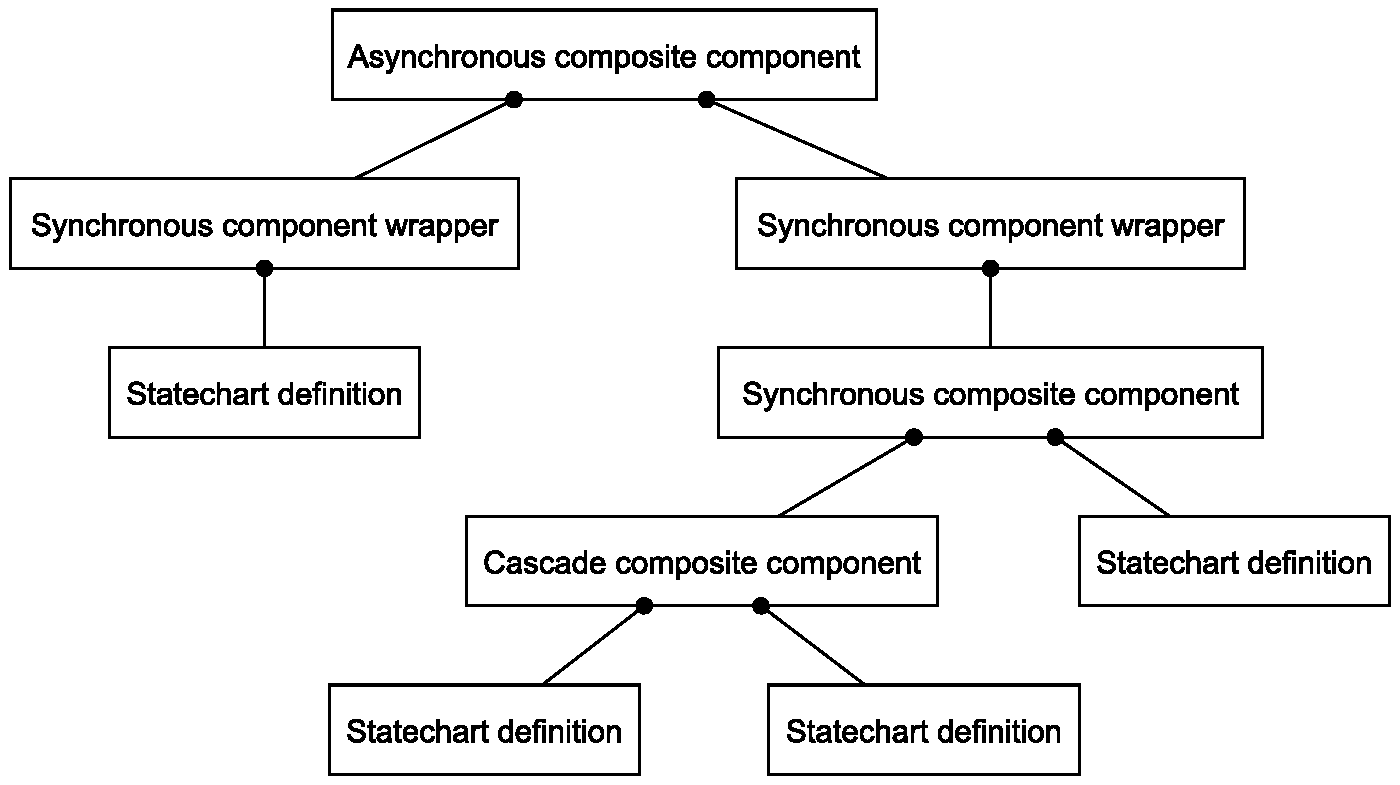
\includegraphics[width=1.0\linewidth]{figures/gamma_object_tree.pdf}
%	%	}
%	\caption{A composite model hierarchy in \gamma.}
%	\label{fig:gamma-object-tree}
%\end{figure}

\section{Conclusion and Future Work}
\label{sec:conclusion}
In this paper, we have proposed an extension to the composition language of the \framework\ to support the mixing of
%a modeling tool that supports the development of reactive systems by offering hierarchical composition of statechart components. 
three semantic variants for the composition of reactive components: asynchronous-reactive, synchronous-reactive and cascade semantics. Asynchronous components represent independently running components, which communicate with messages stored in message queues. This semantics is suitable for designing
distributed or parallel processes. Synchronous-reactive components are useful for modeling a single executing unit consisting of multiple, functionally decomposed components.
This composition mode is for the design of different aspects of a complex, but single-threaded component. Cascade composition is practical for designing units with pipeline-like behavior: the input fed into the model is processed by multiple consecutive filters in a single run.

Subject to future work, we plan to extend the code generation and formal verification services of \gamma\ to support the proposed language and the semantic variants it introduces. For code generation, we already have code templates for the more significant methods. The formal analysis of asynchronous-reactive models, however, will be worth more research, as the interleaving semantics of asynchronous models poses a serious challenge to model checkers that should be handled in the transformation to the formal input models of these tools.

\section*{Acknowledgment}
%\vspace{-0.3cm}
%\begin{figure}[!h]
%	\centering
%	\includegraphics[width=0.10\textwidth]{figures/unkp_logo.jpg}
%\end{figure}
%\vspace{-0.28cm}
Partially supported by the \'UNKP-17-2-I and \'UNKP-17-3-I New National Excellence Program of the Ministry of Human Capacities.



% trigger a \newpage just before the given reference
% number - used to balance the columns on the last page
% adjust value as needed - may need to be readjusted if
% the document is modified later
%\IEEEtriggeratref{8}
% The "triggered" command can be changed if desired:
%\IEEEtriggercmd{\enlargethispage{-5in}}

% references section

% can use a bibliography generated by BibTeX as a .bbl file
% BibTeX documentation can be easily obtained at:
% http://mirror.ctan.org/biblio/bibtex/contrib/doc/
% The IEEEtran BibTeX style support page is at:
% http://www.michaelshell.org/tex/ieeetran/bibtex/
%\bibliographystyle{IEEEtran}
% argument is your BibTeX string definitions and bibliography database(s)
%\bibliography{IEEEabrv,../bib/paper}
%
% <OR> manually copy in the resultant .bbl file
% set second argument of \begin to the number of references
% (used to reserve space for the reference number labels box)
\bibliographystyle{IEEEtran}
\bibliography{IEEEabrv,./bib}


% that's all folks
\end{document}


